\documentclass[a4paper, 12pt]{article}
\usepackage[utf8]{inputenc}
\usepackage[english,russian]{babel}
\usepackage[warn]{mathtext}
\usepackage{graphicx}
\usepackage{float}
\usepackage{multirow}
\restylefloat{table}
\usepackage{amsmath}
\usepackage{floatflt}
\usepackage[T2A]{fontenc}
\usepackage[left=20mm, top=20mm, right=20mm, bottom=20mm, footskip=10mm]{geometry}
\usepackage{amssymb}

\tolerance 1414
\hbadness 1414
\emergencystretch 1.5em
\hfuzz 0.3pt        % размер максимального переполнения без warning'a
\widowpenalty=10000 % запрещает одиночную строку абзаца в начале страницы
\vfuzz \hfuzz
\raggedbottom       % если на странице мало содержимого, добавить пустое место в конце, а не в середине страницы



\begin{document}

\begin{titlepage}
	\centering
	\vspace{5cm}
	{\scshape\LARGE московский физико-технический институт (национальный исследовательский университет) \par}
	\vspace{6cm}
	{\scshape\Large Лабораторная работа 4.3.1 \par}
	{\huge\bfseries Дифракция света \par}
	\vspace{1cm}
	\vfill
\begin{flushright}
	{\large Б03-102}\par
	\vspace{0.3cm}
	{\LARGE Куланов Александр}
\end{flushright}
	

	\vfill


	Долгопрудный, 2023 г.
\end{titlepage}

\begin{itemize}
	\item \textbf{Цель работы:} исследовать явления дифракции Френеля и Фраунгофера на одной и двух щелях, изучить влияние дифракции на разрешающую способность оптических инструментов; проверить теоретические соотношения для положения максимумов при дифракции Френеля и Фраунгофера
    \item \textbf{В работе используются:} оптическая скамья, ртутная лампа, светофильтр, щели с регулируемой шириной, рамка с вертикальной нитью, экран с двойной щелью, микроскоп на поперечных салазках с микрометрическим винтом, зрительная труба
\end{itemize}

\section{Экспериментальная установка}
\subsection*{Дифракция Френеля}

\begin{figure}[H]
    \centering
    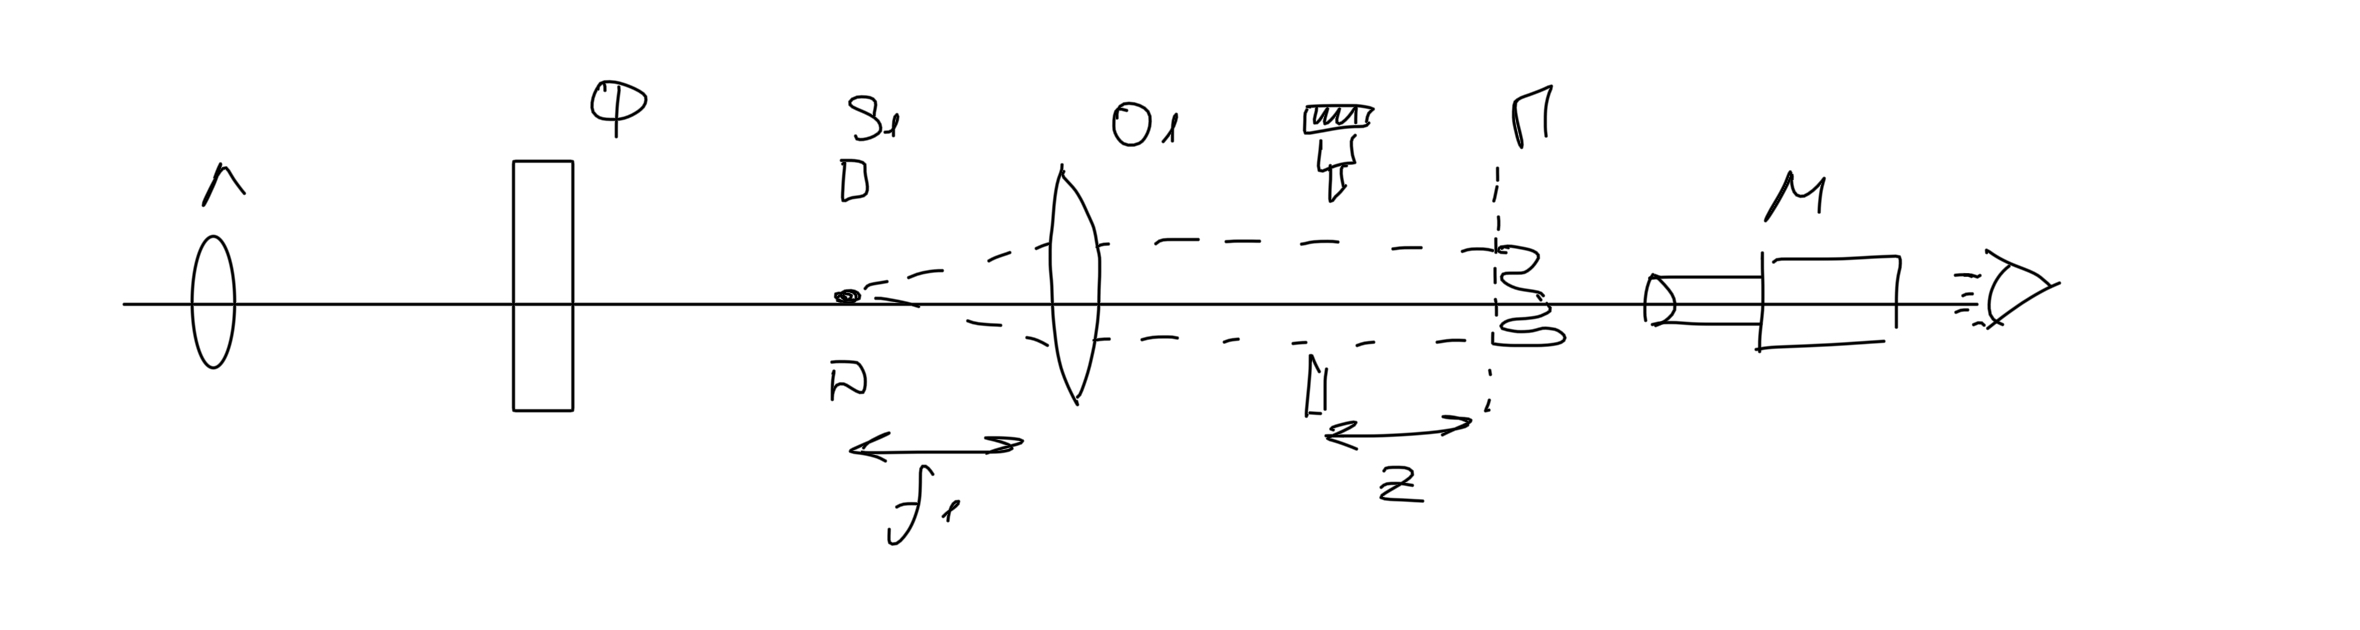
\includegraphics[width=1\textwidth]{frenel.jpg}
    \caption{Дифракция френеля}
    \label{fig:ris1}
\end{figure}

Схема установки для наблодения дифракции Френеля представлена на рис. 1. Свет от ртутной ртутной ламы Л, пропущенный через оранжевый светофильтр $\Phi$ со средней длиной волны $\lambda=578$ нм, падает на входную щель $S_1$. Щель $S_1$ находится в фокусе коллиматора - собирающей линзы $O_1$. Коллиматор создаёт параллельный пучок монохроматического света, освещающий щель $S_2$, на которой и происходит дифракция. Дифракционная картина рассматривается с помощьо микроскопа $M$, сфокусированного на некоторую плоскость наблюдения П.

Распределение интенсивности света в плоскости наблюдения П проще всего рассчитывать с помощыо зон Френеля (для щели их также называют зонами ШIустера). При освещении щели $S_2$ параллельным пучком лучей (плоская волна) зоны Френеля представляют собой полоски, параллельные краям щели. Результирующая амплитуда в точке наблодения определяется суперпозицией колебаний от тех зон Френеля, которые не перекрыты створками щели. Границы зон Френеля/Шустера $\xi_m$ определяется соотношением
$$
\xi_m= \pm \sqrt{m z \lambda}, \quad m \in \mathbb{N}
$$
где $\xi$ отсчитывается от центра щели, $z$ - расстояние от щели до плоскости наблодения П, a $\lambda$ - длина волны. При ширине щели $b(-b / 2<\xi<b / 2)$ полное число открытых зон для точки наблодения на оси равно
$$
m_{\max }=\frac{b^2}{4 \lambda z}
$$

По определению, разделение волнового фронта на зоны Френеля производится так, чтобы излучение от соседних зоны находилось в противофазе. Иными словами, разность хода (от поверхности фронта до точки наблюдения) между краями соседних зон равна $\lambda / 2$. Поэтому, когда открыто чётное число зон Френеля, на оси системы наблюдается минимум дифракционной картины (тёмная полоса). Если число открытых зон нечётно, в центре картины - максимум (светлая полоca).

Зафиксируем размер щели $b$ и проанализируем, как меняется картина в зависимости от расстояния до плоскости наблюдения $z$. Если число открытых зон Френеля велико, $m \gg 1(z \rightarrow 0)$, мы приходим к пределу геометрической оптики. В нём дифракционная картина отсутствует, а размер изображения щели совпадает с шириной самой щели $b$. Дифракционная картина наблюдается только в узкой полосе вблизи границ щели («дифракция на краго экрана»). При удалении от плоскости геометрического изображения эти две группы полос постепенно расширяотея, заполняя всё изображение щели. При $m \sim 1$ на щели наблюдается сложная картина из небольшого числа дифракционных полос. При дальнейшем удалении $(m \ll 1, z \rightarrow \infty)$ дифракционная картина начинает упрощаться и расширяться, переходя в режим Фраунгофера - затухающие по интенсивности эквидистантные полосы c характерным угловым размером центральной полосы $\lambda / b$.

Амплитуду света в произвольной точке плоскости наблодения можно определить графически с помощъю векторной диаграммы - спирали Корню (см. п. 1.4.2 Введения к разделу).

Распределение амплитуд в режиме дифракции Френеля $(m \sim 1)$ довольно сложно. Однако если число открытых зон Френеля больше единицы и близко к целому $m=2,3,4, \ldots$, то в картине можно довольно чётко выделить $m-1$ тёмных полос, заполнягощих изображение щели. Так можно по виду дифракционной картины оценить число зон Френеля на полуширине щели.

\subsection*{Дифракция Фраунгофера на щели}

\begin{figure}[H]
    \centering
    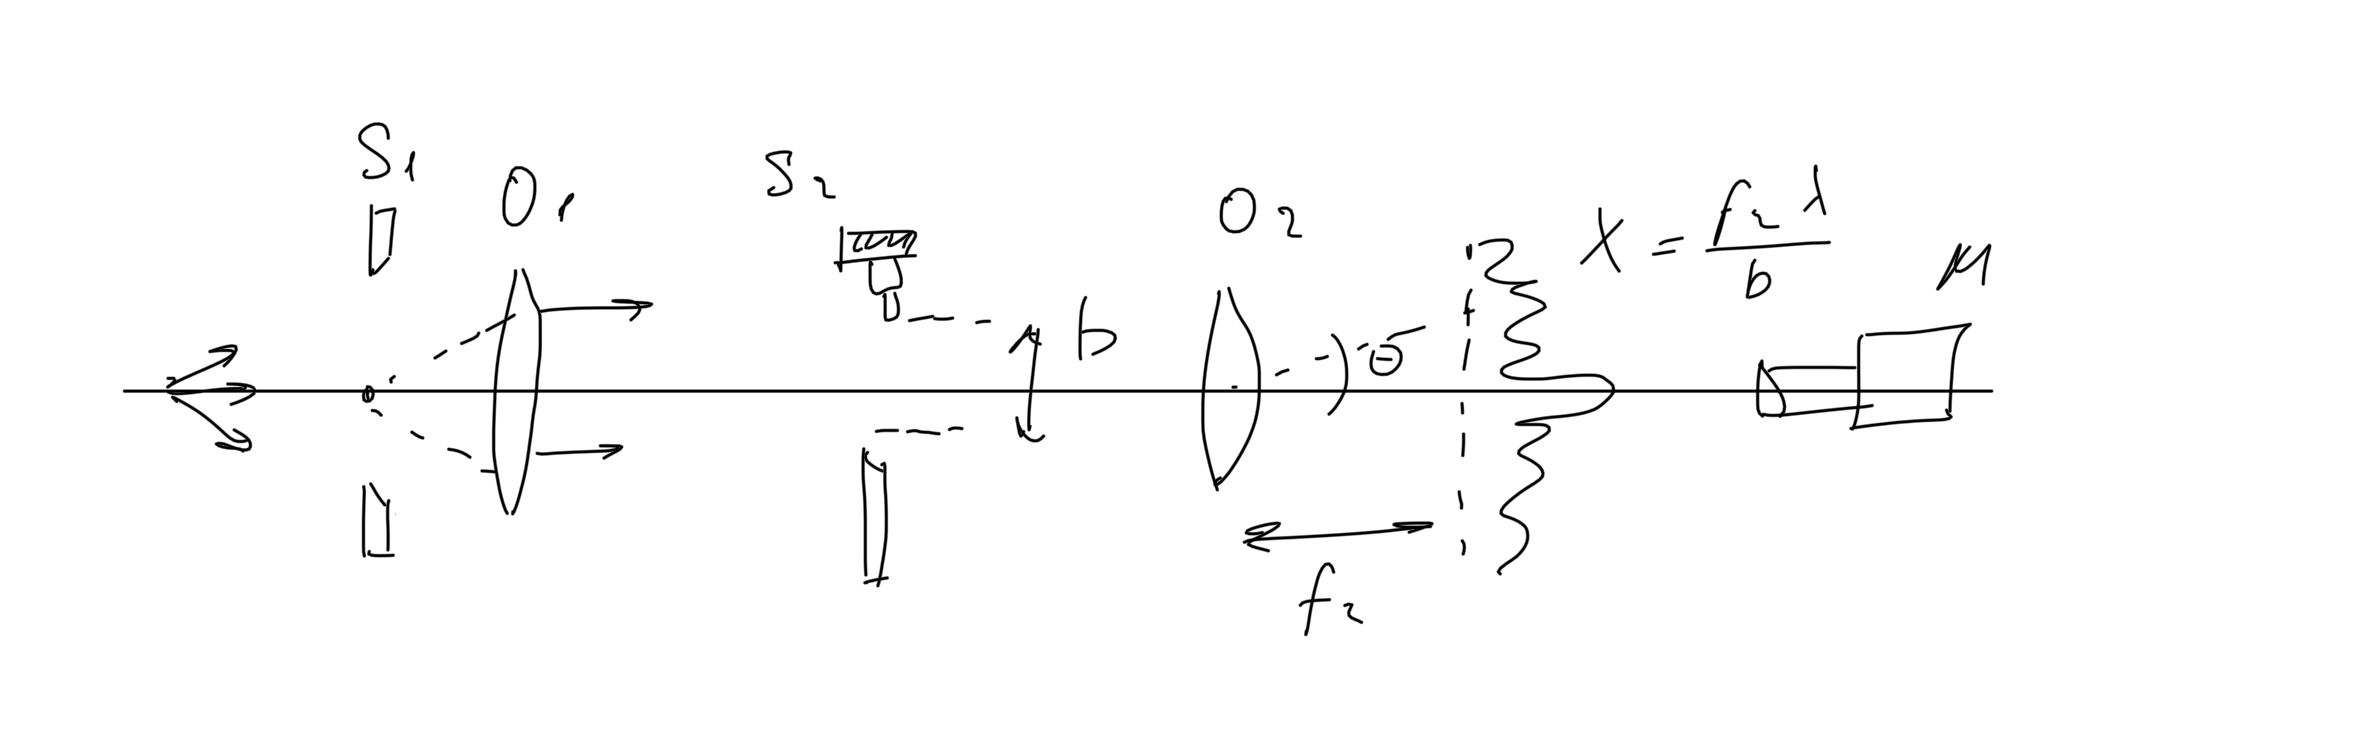
\includegraphics[width=1\textwidth]{fraun1.jpg}
    \caption{Дифракция Фраунгофера на щели}
    \label{fig:ris2}
\end{figure}


На значительном удалении от щели, когда выполнено условие $m \ll 1$ (то есть ширина щели становится значительно меньше ширины первой зоны Френеля, $b \ll \sqrt{\lambda z}$ ), изображение щели размывается и возникает дифракционная картина, называемая дифракцией Фраунгофера.

Дифракцию Фраунгофера можно наблодать той же установке, что и дифракцию Френеля (рис. 1). Однако при обычных размерах установки дифракция Фраунгофера возникает только при очень узких щелях. Поскольку работать с тонкими щелями неудобно, для наблодения дифракции Фраунгофера к схеме добавляется объектив $O_2$ (рис. 3).

Дифракционная картина наблодается в фокальной плоскости объектива $O_2$. Поскольку объектив не вносит дополнительной разности хода между интерферирующими лучами ( таутохронизм тонкой линзы), в его фокальной плоскости наблодается неискажённая дифракционная картина Фраунгофера, соответствующая бесконечно удалённой плоскости наблодения.

При дифракции Фраушофера в центре поля зрения наблодается дифракционный максимум (светлая полоса). Сбоку от неё наблодаются чередующиеся минимумы и максимумы с довольно быстро затухаюощей интенсивностыю. Направление на минимумы (тёмные полосы) ${ }^*$ при малых углах $\Theta$ определяется соотношением
$$
\Theta_n^{\min }=n \frac{\lambda}{b}, \quad n= \pm 1, \pm 2, \ldots,
$$
где $b$ - ширина щели. Каждому значению угла $\Theta$ соответствует точка в плоскости объектива с фокусным расстоянием $f_2$, отстоящая от оптической оси на расстоянии
$$
X_n=f_2 \operatorname{tg} \Theta_n \approx f_2 \Theta_n
$$
Измеряя зависимость $X$ от $m$ или расстояние между полосами $\Delta X$, можно определить ширину щели $S_2$.


\subsection*{Дифракция Фраунгофера на двух щелях}

\begin{figure}[H]
    \centering
    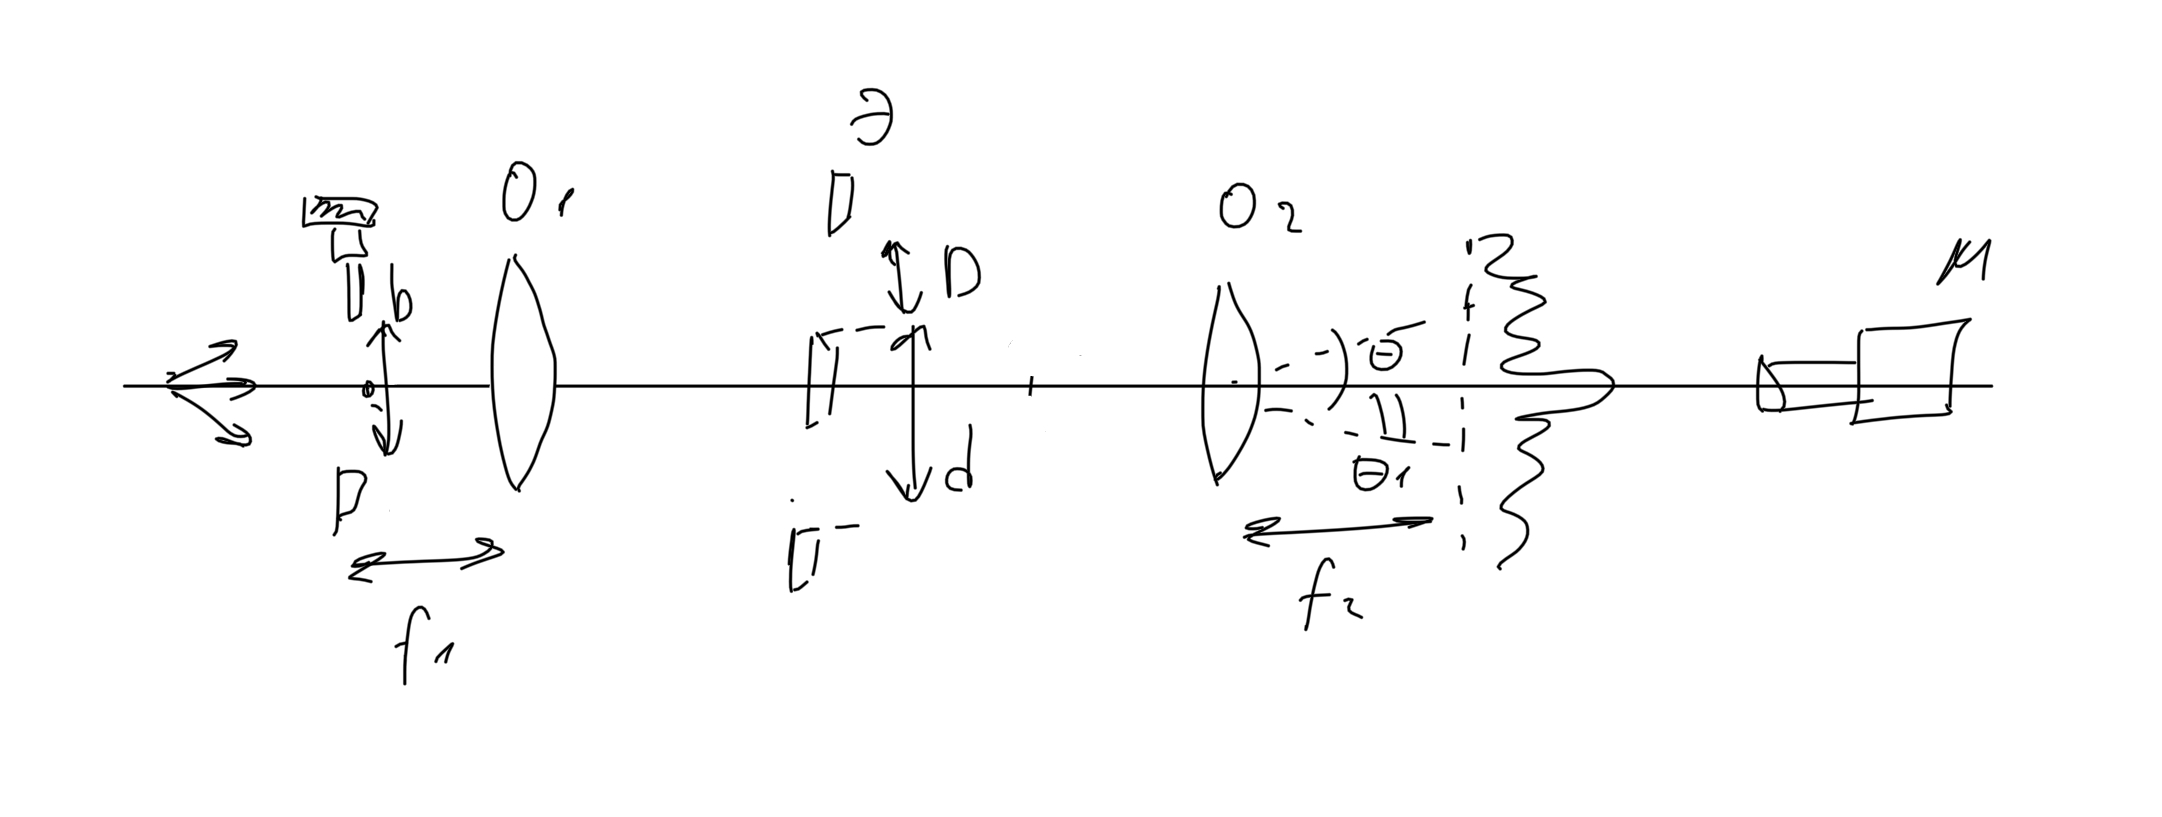
\includegraphics[width=1\textwidth]{fraun2.jpg}
    \caption{Дифракция Фраунгофера на двух щелях}
    \label{fig:ris3}
\end{figure}

Схема для наблодения дифракции Фраунгофера на двух щелях изображена на рис. 4. По сравнению с рис. 3 в ней щель $S_2$ заменена на экран $\ni$ с двумя щелями. При этом щель $S_2$ (с микрометрическим винтом) установлена вместо входной щели $S_1$ (для измерения влияния ширины источника на чёткость картины).

Результат дифракции на двух щелях можно представить как интерференциюо дифракционных картин от каждой щели (аналог интерференционной схемы Юнга).

Если входная щель достаточно узка, то дифракционная картина в плоскости П (рис. 4) подобна той, что получалась при дифракции на одной щели, однако теперь вся картина
испещрена рядом дополнительных узких полос. Наличие этих полос объясняется суперпозицией (интерференцией) световых волн, приходящих в плоскость наблюдения через разные щели экрана $\vartheta$. В центре главного дифракционного максимума располагдется светлая полоса (разность на оси, в силу симметрии, равна нуло). Светлая интерференционная полоса наблодается также, когда разность хода кратна длине волны. Угловая координата $\theta_n$ интерференционного максимума $n$-го порядка определяется соотношением
\begin{equation*}
\theta_n d=n \lambda, \quad n= \pm 1, \pm 2, \ldots
\end{equation*}
где $d$ - расстояние между щелями. Линейное расстояние $\delta x$ между соседними интерференционными полосами в плоскости П равно поэтому
\begin{equation*}
\delta x=f_2 \frac{\lambda}{d}
\end{equation*}
На рис. 4 показано распределение интенсивности в фожальной плоскости объектива $\mathrm{O}_2$. Штриховой линией (в увеличенном масштабе) изображено распределение интенсивности при дифракции света на одиночной щели. Поскольку полная угловая ширина главного дифракционного максимума (от минимума до минимума) равна $2 \lambda / D$, где $D$ - ширина отдельной щели, то на нём укладывается $N=\frac{2 d}{D}$ тёмнъх интерференционных полос (в центре картины максимум, поэтому светлых полос - на одну больше).

При дифракции света на двух щелях чёткая система интерференционных полос наблюдается только при достаточно узкой ширине входной щели $\left(S_2\right)$, которую можно рассматривать как протяжённый источник света размером $b$. Для наблодения интерференции необходимо, чтобы расстояние $d$ между щелями не превышало радиуса когерентности (см. раздел ІІ):
\begin{equation*}
d \leqslant \rho_{\text {Kor }} \approx \frac{\lambda}{b} f_1 .
\end{equation*}
Таким образом, по размытию интерференционной картины можно оценить размер источника b. Этот метод используется в звёздном интерферометре при измерении угловых размеров звёзд.

\subsection*{Влияние дифракции на разрешающую способность оптического инструмента}

\begin{figure}[H]
    \centering
    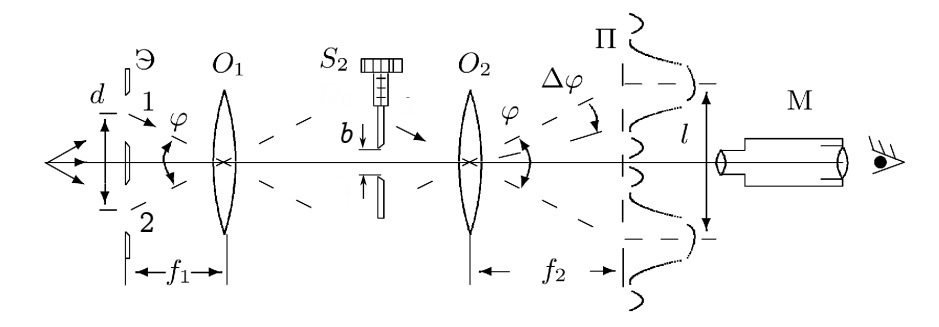
\includegraphics[width=1\textwidth]{razresh.jpg}
    \caption{Влияние дифракции на разрешающую способность оптического инструмента}
    \label{fig:ris4}
\end{figure}

Установка, использованная в упражнении Б (рис. 4), позволяет исследовать влияние дифракции на разрешаюицо способность оптических инструментов.

Линзы $O_1$ и $O_2$ (без щели $S_2$ ) создают в плоскости П изображение щели входной $S_1$, рассматриваемое в микроскоп М. Таким образом, пара линз $O_1, O_2$ и микроскоп в совокупности может рассматриваться как некий оптический инструмент. При этом входная щель $S_1$ и коллиматор $O_1$ создают модель далёкого предмета, а объектив $O_2$ и микроскоп М составляют «зрительную трубу», наведённую на этот предмет.

Если перед объективом $O_2$ зрительной трубы расположить щель $S_2$, то изображение объекта будет искажено дифракцией на щели $S_2$. Чем меньше ширина $b$ этой щели, тем сильнее искажение. Качественной характеристикой этих искажений может служить минимальное угловое расстояние $\varphi$ между точками рассматриваемого предмета, которые воспринимаются как разделънье.

В качестве предмета будем использовать экран $\text{Э}$ с двумя узкими щелями (поместим его вместо щели $S_1$ ). Пусть расстояние между щелями равно $d$. Тогда от каждой из щелей экрана на щель $S_2$ будут падать два параллельных пучка света, составляющих между собой угол
\begin{equation*}
\varphi \approx \frac{d}{f_1}
\end{equation*}
(а центры двух дифракционных пятен в плоскости П будут находиться на расстоянии $l=f_2 \varphi$ друг от друга). ли $S_2$. В режиме дифракции Фраунгофера полуширина центрального дифракционного максимума равна $\Delta \varphi \sim \lambda / b$, где $b$ - ширина щели $S_2$.

Если полуширина главного дифракционного пятна превысит расстояние между центрами пятен $\Delta \varphi>\varphi$, пятна от двух щелей сольются в одно, и по виду дифракционной картины будет трудно определить, представляет ли собой источник двойную или одиночную щель. Это условие разрешения двух изображений называют также жритерием Рэлея. Итак, щели можно считать различимыми, если
\begin{equation*}
\frac{\lambda}{b}<\frac{d}{f_1}
\end{equation*}




\section{Практическая часть}
\subsection{Дифракция Френеля}
Соберем установку на рис. 1. Для этого включим ртутную лампу и поставим после нее фильтр с щелью. После щели нужно будет поставить линзу так, чтобы щель была в фокусе. Для этого воспользуемся зрительной трубой, настроенной на бесконечность. Поскольку, если линза находится в нужном месте, из нее выходит пучок параллельных лучей, зрительная труба, настроенная на бесконечность, должна показать четкое изображение щели. После установки линзы поместим щель $S_2$ и микроскоп после неё.
Найдем нуль микрометрического винта щели $S_2$. Для этого посмотрим свозь щель на лампу накаливания и начнем поворачивать винт из нулевого положения до тех пор, пока свет от лампы не станет виден. При этом положение винта будет нулем.

\begin{center}
\begin{tabular}{|c|c|c|c|}
\hline
$d, \text{мкм}$&$57$&$56$&$56$\\ \hline
\end{tabular}\\~\\
\end{center} 
\[<d> = 56.3 \pm 1.0\; \text{мкм}\]

Измерим положение микроскопа $x$, при котором видно $n$ полос и найдем расстояние $a$ до плоскостии наблюдения, которое равно смещению относительно положения $x_0=88.0\pm0.5\,\text{мм}$

\begin{table}[H]
\begin{center}
\begin{tabular}{|c|c|c|c|c|c|}\hline
$m$ & $x_{min}\text{, \text{мм}}$ & $x_{max}\text{, \text{мм}}$ & $ a\text{, \text{мм}}$&$\Delta a\text{, \text{мм}}$&$2\xi \text{, \text{мм}}$\\\hline
$1$ & $56.0$ & $54.0$ & $2$ &$0.1$&$0.11$\\\hline
$2$ & $50.5$ & $48.0$ & $2.5$ &$0.1$&$0.165$\\\hline
$3$ & $44.5$ & $43.0$ & $1.5$ &$0.1$&$0.15$\\\hline
$4$ & $41.0$ & $40.5$ & $0.5$ &$0.1$&$0.1$\\\hline
$5$ & $39.5$ & $38.5$ & $1.0$ &$0.1$&$0.15$\\\hline
\end{tabular}\\~\\
\end{center}
\caption{\label{tab:first}}
\end{table}

Ширина щели: $b = (0.15 \pm 0.05)\; \text{мм}$

% \begin{figure}[H]
% 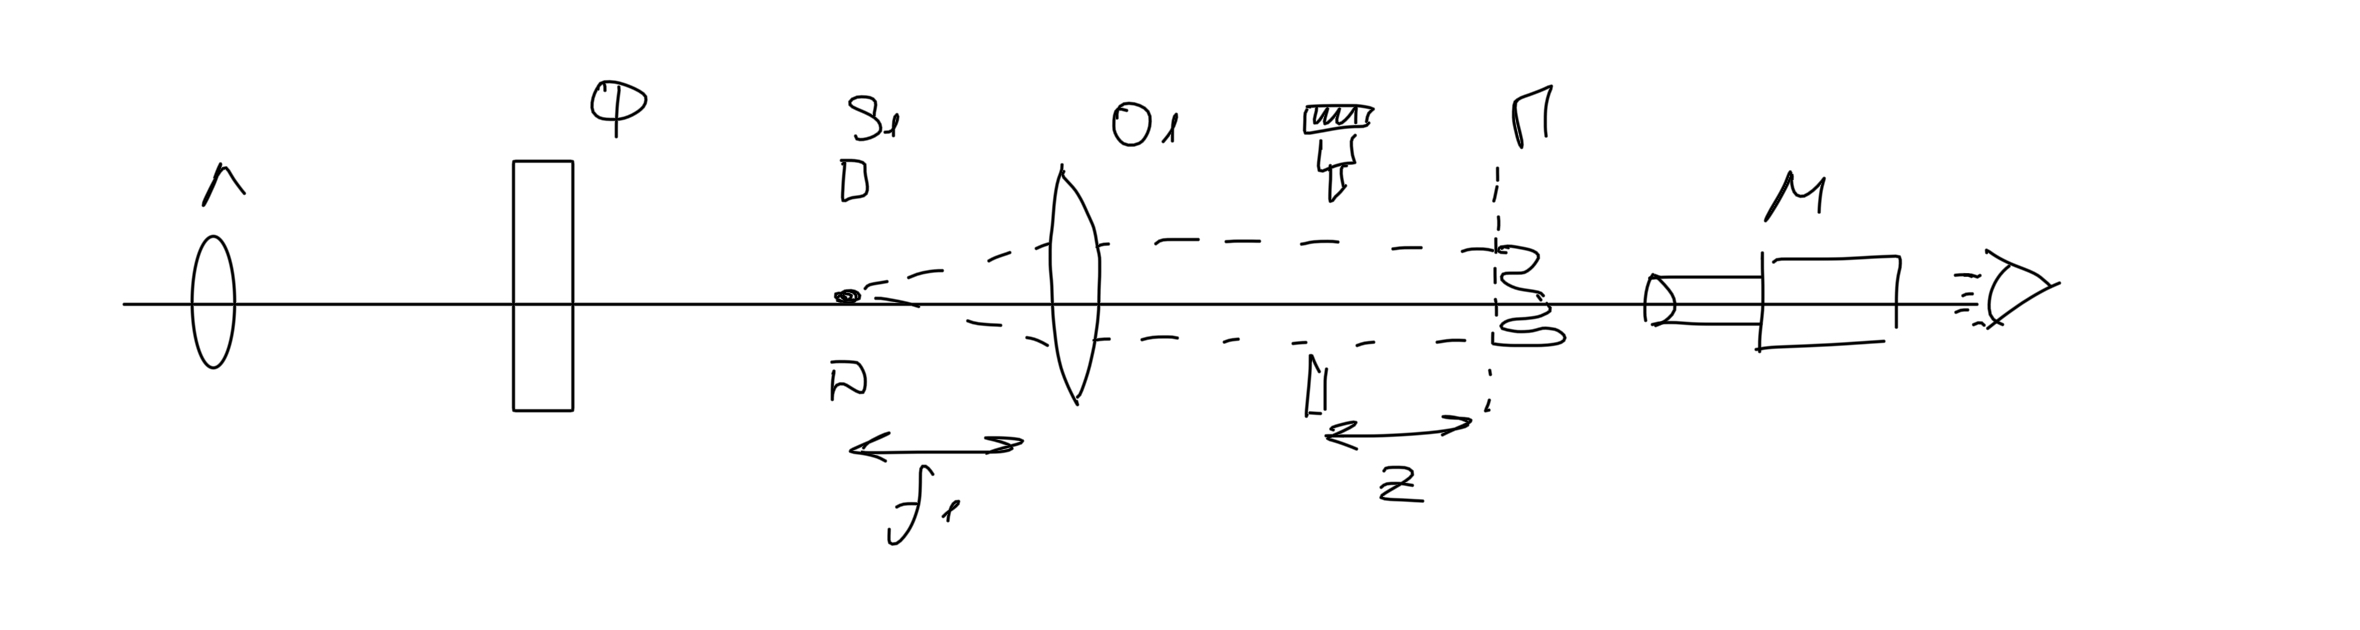
\includegraphics[scale=0.9]{frenel.png}
% \end{figure}

Все результаты повторно сравниваются в выводах лабораторной работы.

\subsection{Дифракция Фраунгофера}

Фокусные расстояния линз: $F_1 = 11.5$ и $F_2 = 12.5$.

Ширина щели: $b = (0.303 \pm 0.05) \text{мм}$

Цена деления: 0.02 мм

Возьмём половину дифракционной картины Фраунгофера, так как можно получить данные до 6 порядка включительно (вторая половина аналогична). Рассчитаем также ширину щели по формуле (7):

\begin{table}[H]
\begin{center}
\begin{tabular}{|c|c|c|c|c|c|}\hline
$m$ & $Divisions$ & $x_m, \text{мм}$ & $\sigma(x_m), \text{мм}$ & $b, \text{мм}$ & $\sigma(b), \text{мм}$\\\hline
$1$ & $11$  & $0.22$ & $0.01$ & $ 0.310$ & 0.02\\\hline
$2$ & $23.5$ & $0.47$ & $0.01$ & $0.291$ & 0.02\\\hline
$3$ & $35.5$ & $0.71$ & $0.01$ & $0.288$ & 0.02\\\hline
$4$ & $47$ & $0.94$ & $0.01$ & $0.291$ & 0.02\\\hline
$5$ & $59$ & $1.18$ & $0.01$ & $0.289$ & 0.02\\\hline
$6$ & $68$ & $1.36$ & $0.01$ & $0.301$ & 0.02\\\hline
\end{tabular}\\~\\
\end{center}
\caption{\label{tab:second}}
\end{table}

Здесь расстояние $x_m$ - расстояние от оптической оси объектива до середины чёрной полосы.

Построим график зависимости этого расстояния от порядка $m$.

\begin{figure}[H]
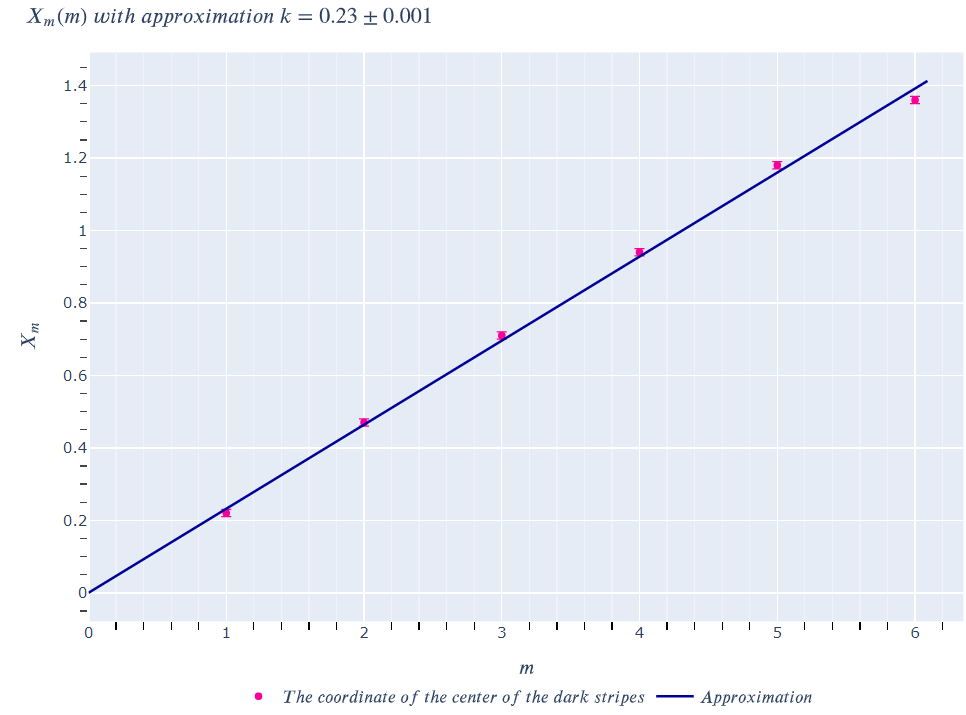
\includegraphics[scale=0.9]{Fraunhofer.png}
\end{figure}

Из графика  $k = 0.23$ - коэффициент наклона и есть $\Delta x$ - среднее расстояние между соседними минимумами.

Из Таблицы \ref{tab:second} $b_{\text{ср}} = 0.295\; \text{мм}$ 

Сделаем ещё один эксперимент с другой шириной щели, возьмём максимальную ширину щели $b = 4.0\; \text{мм}$

\begin{table}[H]
\begin{center}
\begin{tabular}{|c|c|c|c|c|c|}\hline
$m$ & $Divisions$ & $x_m, \text{мм}$ & $\sigma(x_m), \text{мм}$ & $b, \text{мм}$ & $\sigma(b), \text{мм}$\\\hline
$1$ & $9$  & $0.18$ & $0.01$ & $ 0.379$ & 0.02\\\hline
$2$ & $17$ & $0.34$ & $0.01$ & $0.402$ & 0.02\\\hline
$3$ & $27$ & $0.54$ & $0.01$ & $0.379$ & 0.02\\\hline
$4$ & $31.5$ & $0.63$ & $0.01$ & $0.433$ & 0.02\\\hline
$5$ & $41.5$ & $0.83$ & $0.01$ & $0.411$ & 0.02\\\hline
$6$ & $57.5$ & $1.15$ & $0.01$ & $0.356$ & 0.02\\\hline
$7$ & $72$ & $1.44$ & $0.01$ & $0.379$ & 0.02\\\hline
\end{tabular}\\~\\
\end{center}
\caption{\label{tab:third}}
\end{table}

% \begin{figure}[H]
% \includegraphics[scale=0.9]{Fraunhofer4.png}
% \end{figure}

Из графика  $k = 0.19$ -  $\Delta x$ - среднее расстояние между соседними минимумами.

Из Таблицы \ref{tab:second} $b_{\text{ср}} = 0.391\; \text{мм}$ 


\subsection{Дифракция фраунгофера на 2-х щелях}

Измерим ширину главных максимума, посчитаем количество тёмных полос
\begin{equation*}
    X = (0.52 \pm 0.01)\; \text{мм}
\end{equation*}
\begin{equation*}
    n = 11
\end{equation*}
\begin{equation*}
    \delta x = \frac{X}{n}
\end{equation*}
\begin{equation*}
    \delta x = (0.047 \pm 0.001)\; \text{мм}
\end{equation*}

Тогда расстояние между щелями, считается по формуле (7):
\begin{equation*}
    d = (1.45 \pm 0.03)\; \text{мм}
\end{equation*}

Сравним результаты с теоретическими:
\begin{equation*}
    d = (1,00 \pm 0.01)\; \text{мм}
\end{equation*}
\begin{equation*}
    D = (0,180 \pm 0.01)\; \text{мм}
\end{equation*}

Тогда количество светлых полос по теории:
\begin{equation*}
    n = 11
\end{equation*}

\subsection{Влияние дифракции на разрешающую способность
оптического инструмента}
Подберём ширину щели так, чтобы изображения обеих щелей почти сливались, но всё-таки ещё воспринимались раздельно.
\begin{equation*}
    b = 0.284
\end{equation*}
Сравнивая с формулой для критерия Релея, имеем пропорциональность, соответсвенно дифракционные пятна различимы.


\subsection{Вывод} 
Про суть явления: реальных вторичных источников нет, это удобный способ восприятия. Все что видно в дифракции, связано исключительно с наличием вещества, первичное излучение взаимодействует с молекулами из которых состоят границы щели, оно начинает переизлучать, оно же идет в разные стороны и именно его мы и наблюдаем.

Приведём таблицу полученных экспериментальных данных:
\begin{center}
\begin{table}[h]
\begin{tabular}{|c|c|c|c|c|c|}
\hline
                & \begin{tabular}[c]{@{}c@{}}Дифракция \\ Френеля\end{tabular} & \begin{tabular}[c]{@{}c@{}}Дифракция \\ Фраунгофера\\ на одной щели (1)\end{tabular} & \begin{tabular}[c]{@{}c@{}}Дифракция \\ Фраунгофера\\ на одной щели (2)\end{tabular}   &             
                & \begin{tabular}[c]{@{}c@{}}Дифракция \\ Фраунгофера\\ на двух щелях\end{tabular} \\ \hline
$D_{theor}$, мм & $0,15\pm 0,01$                                                          & $0,303 \pm 0,01$ & $0,4 \pm 0,01$ & $d_{theor}$, мм & $1,00\pm0,01$\\ 
\hline
$D_{prac}$, мм  & $0,16\pm 0,03$                                                        & $0,295\pm 0,02$                                                                            &  $0,391 \pm 0,02$ & $d_{prac}$, мм  & $1,45\pm0,03$                                                                             \\ \hline
\end{tabular}
\end{table}
\end{center}
Для лучшего понимания, был сделан второй эксперимент с дифракцией Фраунгофера. Также приводится схематичный график сравнения интенсивностей:

% \centering
% \begin{figure}[H]
% \includegraphics[scale=0.7]{intense.png}
% \end{figure}
% \centering

\end{document}